\chapter{Metodologia}

Introduzir o capitulo de Metodologia - sobre o que falaremos.

\section{Termo de Abertura do Projeto - TAP}

Trazer o TAP.

\section{Estrutura Analítica do Projeto (EAP)}

Trazer e explicar a EAP do projeto - com respeito aos pontos de controle.

\section{Comunicação}

Explicar o método que o time utilizou para se comunicar - ferramentas, reuniões, etc.

\section{Custos}

Explicar o método que utilizaremos para gerenciar os custos.

\section{Tempo}

Explicar o método que utilizaremos para lidar com o tempo - falar do cronograma.

\section{Recursos Humanos}

Explicar como organizamos os papeis.

\section{Requisitos}

Explicar como gerenciaremos os requisitos do projeto.

\section{Riscos}

Explicar como gerenciaremos e mitigaremos os riscos.

\section{Desenvolvimento do Relatório}

A confecção do relatório será dividida em dois fluxos - um geral, onde o
conteúdo será escrito e revisado, e a implantação no relatório, onde um
membro que domine \LaTeX\ e
Git\footnote{\url{https://git-scm.com/}} transcreverá o conteúdo para o
relatório final.

\subsection{Fluxo 1 - Criação do conteúdo}

\begin{figure}[H]
  \centering
    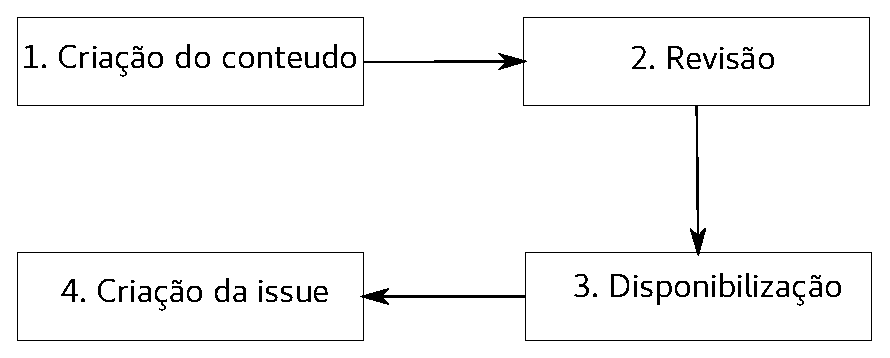
\includegraphics[width=\textwidth]{figuras/fluxo1.eps}
  \caption{Fluxo 1 - Criação do conteúdo.}
  \label{fig:fluxo1}
\end{figure}

\begin{enumerate}
  \item O conteúdo é escrito, de maneira formatada e com referências;
  \item O conteúdo é revisado pelo seu autor, que corrigirá defeitos encontrados;
  \item O autor disponibiliza o conteúdo em algum meio acessível pelos outros membros;
  \item O autor cria uma \textit{issue} no repositório do
    relatório\footnote{\url{https://github.com/CadeiraCuidadora/relatorio}}, explica brevemente
    o conteúdo criado, e disponibiliza o \textit{link} para o conteúdo. A \textit{issue} deverá ser associada a \textit{label} de relatório.
\end{enumerate}

\subsection{Fluxo 2 - Implantação no Relatório}

\begin{enumerate}
  \item Um membro que domine Git e \LaTeX\ encontra uma \textit{issue} que deseja
  implantar no relatório;
  \item Revisa o conteúdo, e o transcreve para o relatório;
  \item Relata na \textit{issue} associada se algum problema ocorreu, ou se terminou a transcrição;
  \item Cria um \textit{merge request} para a \textit{branch master} no repositório;
  \item Outro membro revisa o \textit{merge request}, e aceita ou relata as correções a serem feitas.
\end{enumerate}

